\chapter{The Periodic Table: A First Look}\label{ch:g9:periodic-table-first-look}

On the wall of almost every chemistry classroom hangs the same chart: 118
boxes, each with a symbol and a number, arranged in rows and columns
with a strange shape --- tall towers at the sides, a dip in the middle,
two loose rows below. When it was first drawn, in 1869, it had about
sixty boxes and several empty ones. Its author was bold enough to
describe the elements that would one day fill the gaps --- and he was
right.

\begin{recall}
A \omterm{def:g9:inside-the-atom:element}{chemical element} is the set of \omterm{def:g7:atoms-and-molecules:atom}{atoms} with the same \omterm{def:g9:inside-the-atom:atomic-number}{atomic number} $Z$,
the number of \omterm{def:g9:inside-the-atom:proton}{protons} in the \omterm{def:g9:inside-the-atom:nucleus}{nucleus} (\cref{ch:g9:inside-the-atom}).
Each element has a symbol, one capital letter sometimes followed by a
small one (\cref{ch:g7:atoms-and-molecules}). \omterm{def:g9:periodic-table-first-look:metal}{Metals} such as iron, zinc
and aluminium give positive \omterm{def:g9:ions:ion}{ions} (\cref{ch:g9:ions}).
\end{recall}

\section{A table of the elements}

\begin{definition}[Periodic table]\label{def:g9:periodic-table-first-look:periodic-table}
The \emph{periodic table}\index{periodic table} lists all the \omterm{def:g9:inside-the-atom:element}{chemical
elements} in order of increasing \omterm{def:g9:inside-the-atom:atomic-number}{atomic number}, $Z = 1$ to $Z = 118$,
arranged in rows so that elements with similar properties fall in the
same column.
\end{definition}

\begin{definition}[Period and group]\label{def:g9:periodic-table-first-look:period}
A row of the \omterm{def:g9:periodic-table-first-look:periodic-table}{periodic table} is a \emph{period}\index{period}; there are
seven. A column is a \emph{group}\index{group}; there are eighteen,
numbered 1 to 18 from left to right. The two rows printed below the
table belong in periods 6 and 7; they are set apart only to keep the
table narrow.
\end{definition}

\begin{omfigure}
\omperiodictable[colour=metals, legend=true, cell=0.86cm]

{\small The \omterm{def:g9:periodic-table-first-look:periodic-table}{periodic table}. Each box gives the \omterm{def:g9:inside-the-atom:atomic-number}{atomic number} and the
symbol. Colours: \omterm{def:g9:periodic-table-first-look:metal}{metals}, metalloids (elements between \omterm{def:g9:periodic-table-first-look:metal}{metals} and
\omterm{def:g9:periodic-table-first-look:metal}{non-metals}) and \omterm{def:g9:periodic-table-first-look:metal}{non-metals}, in the usual classification.}
\end{omfigure}

\begin{method}[Reading the periodic table]\label{met:g9:periodic-table-first-look:read}
To place an element:
\begin{enumerate}
  \item find its box from its symbol or its \omterm{def:g9:inside-the-atom:atomic-number}{atomic number};
  \item its row gives its \omterm{def:g9:periodic-table-first-look:period}{period}, its column its group;
  \item its colour says whether it is a \omterm{def:g9:periodic-table-first-look:metal}{metal} or a \omterm{def:g9:periodic-table-first-look:metal}{non-metal}.
\end{enumerate}
Sodium, \ce{Na}, $Z = 11$: \omterm{def:g9:periodic-table-first-look:period}{period} 3, \omterm{def:g9:periodic-table-first-look:period}{group} 1, a \omterm{def:g9:periodic-table-first-look:metal}{metal}. Chlorine,
\ce{Cl}, $Z = 17$: \omterm{def:g9:periodic-table-first-look:period}{period} 3, \omterm{def:g9:periodic-table-first-look:period}{group} 17, a \omterm{def:g9:periodic-table-first-look:metal}{non-metal}.
\end{method}

\section{Metals and non-metals}

\begin{definition}[Metal and non-metal]\label{def:g9:periodic-table-first-look:metal}
A \emph{metal}\index{metal} is an element that, as a \omterm{def:g6:pure-substances-and-mixtures:pure-substance}{pure substance}, is
shiny when freshly cut, conducts electricity and heat well, can be bent
or hammered into shape, and forms positive \omterm{def:g9:ions:ion}{ions}. A
\emph{non-metal}\index{non-metal} lacks these properties: many are gases
(oxygen, nitrogen, chlorine), the solid ones are dull and brittle
(sulfur, carbon as coal), and they tend to form negative \omterm{def:g9:ions:ion}{ions} or to share
\omterm{def:g9:inside-the-atom:nucleus}{electrons} in \omterm{def:g7:atoms-and-molecules:molecule}{molecules}.
\end{definition}

\begin{proposition}[Where they sit]\label{prop:g9:periodic-table-first-look:where}
About four elements in five are \omterm{def:g9:periodic-table-first-look:metal}{metals}; they fill the left and the
centre of the table. The \omterm{def:g9:periodic-table-first-look:metal}{non-metals} sit at the top right, with hydrogen
alone at the top left. Along the border between them, a few elements
--- boron, silicon, germanium, arsenic, antimony, tellurium --- have
properties in between: the metalloids.
\end{proposition}

\section{Columns that behave alike}

\begin{proposition}[Elements of a group behave alike]\label{prop:g9:periodic-table-first-look:alike}
The elements of one group react in similar ways and form similar
compounds. Lithium, sodium and potassium, at the top of \omterm{def:g9:periodic-table-first-look:period}{group} 1, are
soft \omterm{def:g9:periodic-table-first-look:metal}{metals} that react with water, giving off hydrogen; the reaction is
more violent down the group. Fluorine, chlorine, bromine and iodine, in
\omterm{def:g9:periodic-table-first-look:period}{group} 17, are coloured \omterm{def:g9:periodic-table-first-look:metal}{non-metals} that react with \omterm{def:g9:periodic-table-first-look:metal}{metals} to form salts.
Helium, neon, argon and the other elements of \omterm{def:g9:periodic-table-first-look:period}{group} 18 hardly react
with anything.
\end{proposition}

\begin{inthelab}[Lithium, sodium and potassium in water]
Behind a safety screen, the teacher drops a piece of lithium the size of
a grain of rice into a large bowl of water: it fizzes gently. A piece of
sodium the same size whizzes around the surface, melting into a silvery
ball. Potassium bursts into a lilac flame at once. All three give off
hydrogen and leave a \omterm{def:g9:acids-bases-ph:acidic}{basic solution}.
\end{inthelab}

\begin{safety}{\ghs[0.82cm]{GHS02}\ghs[0.82cm]{GHS05}}
% ledger: ghs:Na
Sodium: in contact with water it releases flammable gases which may
ignite (GHS02); it causes severe burns (GHS05). It is kept under oil and
handled only by the teacher, with tongs, in tiny pieces.
\end{safety}

\section{Mendeleev's idea}

\begin{history}[Mendeleev's gaps, 1869--1886]
In 1869 Dmitri Mendeleev arranged the elements then known in order of
increasing atomic weight --- the mass of their \omterm{def:g7:atoms-and-molecules:atom}{atoms} compared with that
of hydrogen --- and placed those with similar properties side by side.
Where the pattern demanded it, he left gaps for elements nobody had yet
found, and in 1871 he described their properties: below silicon, an
``eka-silicon'' whose atomic weight would be about 72. In 1886 the
chemist Clemens Winkler discovered germanium in a silver \omterm{def:g5:raw-materials-and-recycling:raw-material}{ore}, measured
its atomic weight as 72.3 and found it to be the missing element.
Gallium (1875) and scandium (1879) also filled gaps Mendeleev had left.
\end{history}

\begin{omfigure}
\begin{minipage}[b]{0.32\linewidth}\centering
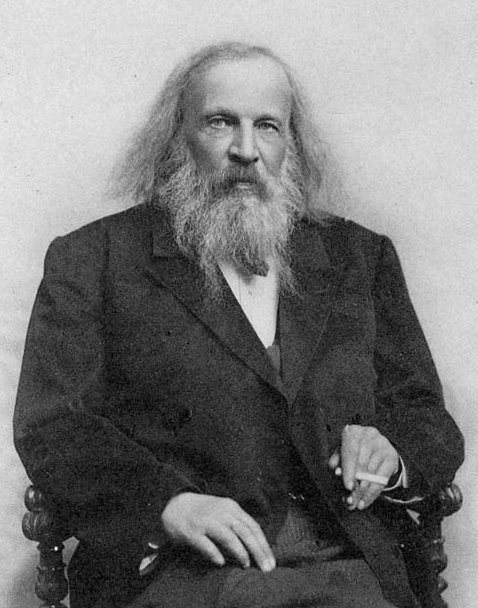
\includegraphics[width=\linewidth]{images/book1/mendeleev.jpg}

{\small Dmitri Mendeleev (1834--1907).}
\end{minipage}\hfill
\begin{minipage}[b]{0.6\linewidth}\centering
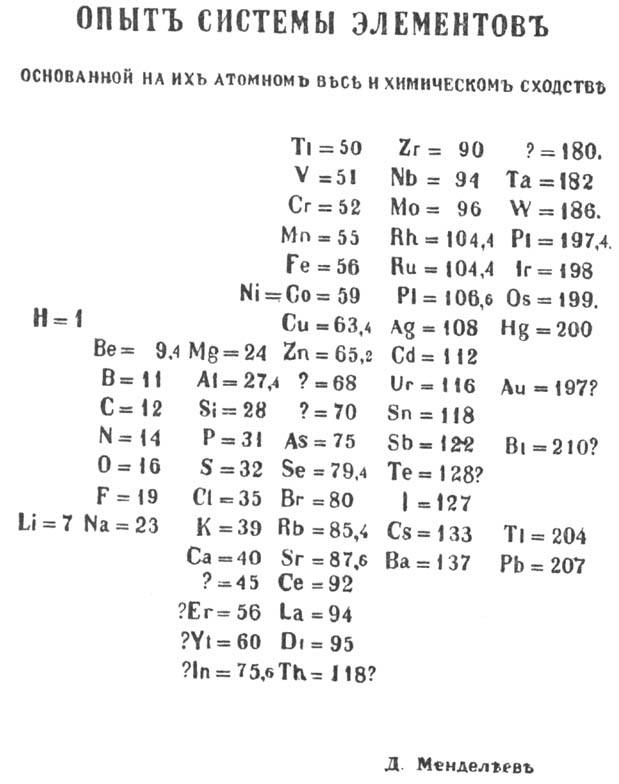
\includegraphics[width=0.85\linewidth]{images/book1/mendeleev-1869.jpg}

{\small Mendeleev's table of 1869, in Russian. Next to Si $= 28$ and
Al $= 27.4$, the gaps ``? $= 70$'' and ``? $= 68$'' wait for germanium
and gallium.}
\end{minipage}
\end{omfigure}

\begin{remark}[Order by atomic number]\label{rem:g9:periodic-table-first-look:order}
Mendeleev ordered the elements by atomic weight, and had to swap a few
pairs, such as tellurium and iodine, to keep the families together.
Today the table is ordered by \omterm{def:g9:inside-the-atom:atomic-number}{atomic number}, discovered later, and the
swaps are no longer needed.
\end{remark}

\section{Exercises}

\begin{exercise}[$\star$]\label{exo:g9:periodic-table-first-look:1}
In what order are the elements placed in the \omterm{def:g9:periodic-table-first-look:periodic-table}{periodic table}?
\end{exercise}

\begin{exercise}[$\star$]\label{exo:g9:periodic-table-first-look:2}
Give the \omterm{def:g9:periodic-table-first-look:period}{period} and the group of: carbon ($Z = 6$), magnesium ($Z = 12$),
argon ($Z = 18$).
\end{exercise}

\begin{exercise}[$\star$]\label{exo:g9:periodic-table-first-look:3}
\omterm{def:g9:periodic-table-first-look:metal}{Metal} or \omterm{def:g9:periodic-table-first-look:metal}{non-metal}: iron, sulfur, copper, oxygen, aluminium, chlorine?
\end{exercise}

\begin{exercise}[$\star$]\label{exo:g9:periodic-table-first-look:4}
Which element is just below sodium in the table? Just below chlorine?
\end{exercise}

\begin{exercise}[$\star\star$]\label{exo:g9:periodic-table-first-look:5}
Using the table, name the element of \omterm{def:g9:periodic-table-first-look:period}{period} 4 and \omterm{def:g9:periodic-table-first-look:period}{group} 2, and the
element of \omterm{def:g9:periodic-table-first-look:period}{period} 2 and \omterm{def:g9:periodic-table-first-look:period}{group} 15.
\end{exercise}

\begin{exercise}[$\star\star$]\label{exo:g9:periodic-table-first-look:6}
Why can one expect potassium to react with water, as sodium does?
\end{exercise}

\begin{exercise}[$\star\star$]\label{exo:g9:periodic-table-first-look:7}
A shiny element conducts electricity and forms the \omterm{def:g9:ions:ion}{ion} \ce{X^{2+}}. Is it
a \omterm{def:g9:periodic-table-first-look:metal}{metal} or a \omterm{def:g9:periodic-table-first-look:metal}{non-metal}? Explain.
\end{exercise}

\begin{exercise}[$\star\star$]\label{exo:g9:periodic-table-first-look:8}
Why did Mendeleev leave gaps in his table? Why was this a strength of his
table rather than a weakness?
\end{exercise}

\begin{exercise}[$\star\star$]\label{exo:g9:periodic-table-first-look:9}
Look at Mendeleev's table of 1869. Which atomic weights did he give for
carbon and for oxygen? Which two gaps, marked with a question mark,
appear next to aluminium and silicon?
\end{exercise}

\begin{exercise}[$\star\star$]\label{exo:g9:periodic-table-first-look:10}
How many elements are there in \omterm{def:g9:periodic-table-first-look:period}{period} 2? In \omterm{def:g9:periodic-table-first-look:period}{period} 4?
\end{exercise}

\begin{exercise}[$\star\star\star$]\label{exo:g9:periodic-table-first-look:11}
Helium, neon and argon hardly react with anything. In which group are
they? What could they be used for, given this property?
\end{exercise}

\begin{exercise}[$\star\star\star$]\label{exo:g9:periodic-table-first-look:12}
Gallium, under aluminium, was discovered in 1875. Mendeleev had predicted
for it an atomic weight close to the average of its neighbours aluminium
(27.0) and indium (114.8). Compute that average. (Gallium: 69.7.)
\end{exercise}

\section{Problem: Mendeleev's Gap}

\begin{problem}[{Weekend problem --- predicting the atomic weight of a
missing element from its four neighbours}]
\label{pb:g9:periodic-table-first-look:1}
% ledger: aw:Si, aw:Sn, aw:Ga, aw:As, aw:Ge, mend:eka-si-aw, ge:winkler-aw
In 1871 Mendeleev predicted the properties of eka-silicon, the element
missing below silicon. One of his ideas was that an element's properties
lie between those of its neighbours above and below, to the left and to
the right. Today's atomic weights of the four neighbours of the gap are:
silicon 28.1 (above), tin 118.7 (below), gallium 69.7 (left), arsenic
74.9 (right).

\medskip
\noindent\textbf{Part I --- The gap.}
\begin{enumerate}
  \item Using the \omterm{def:g9:periodic-table-first-look:periodic-table}{periodic table} of this chapter, find the \omterm{def:g9:inside-the-atom:atomic-number}{atomic number},
        the \omterm{def:g9:periodic-table-first-look:period}{period} and the group of germanium, the element that fills
        the gap.
  \item Which element is above it, which below, which on its left, which
        on its right?
  \item Is germanium a \omterm{def:g9:periodic-table-first-look:metal}{metal}, a \omterm{def:g9:periodic-table-first-look:metal}{non-metal} or a metalloid?
  \item Why did Mendeleev expect the missing element to resemble
        silicon?
\end{enumerate}

\medskip
\noindent\textbf{Part II --- Averages.}
\begin{enumerate}[resume]
  \item Compute the average of the atomic weights of the elements above
        and below the gap.
  \item Compute the average of the atomic weights of the elements on the
        left and on the right.
  \item Which of the two averages is closer to the true atomic weight of
        germanium, 72.6? Why might that be?
  \item In his 1869 table, Mendeleev had written ``? $= 70$'' for this
        gap. By how much was he off?
\end{enumerate}

\medskip
\noindent\textbf{Part III --- The prediction.}
\begin{enumerate}[resume]
  \item Compute the average of all four neighbours, to one decimal
        place.
  \item In 1871 Mendeleev predicted 72; in 1886 Winkler measured 72.3.
        Compare with your average.
  \item Why did the discovery of germanium convince many chemists that
        Mendeleev's table was right?
  \item State your prediction: the atomic weight of eka-silicon from the
        average of its four neighbours.
\end{enumerate}
\end{problem}
